\newpage
\section{Execution and Results} \label{sec:results}
    \subsection{Optimization of Settings}
    Before we started with the actual measurements, we optimized the settings.
    First of all, the parameter $\Delta m$, the resolution \texttt{res} and acceleration voltage $U$ had to be chosen optimally. Additionally, the two detector types Faraday and SEM were compared. The residual gas spectrum of the vacuum chamber was recorded for different settings. Since we assume that the residual gas consists primarily of air, we excluded atoms heavier than 50~amu and limited our scans to the range of 1 to 50 amu. For the step sizes we chose 0.2 amu and carried out 7 measurement runs. If nothing else is written, 70 V was selected as $U$.
    
    $\Delta m$ setting affects the offset of the line. To optimize $\Delta m$ we set \texttt{res} = 0\% and performed measurements for $\Delta m = -10\%, -5\%, 0\%, 5\%, 10\%, 15\%, 20\%, 35\%$.  The curves for $\Delta m = -10\%, 5\%, 20\%, 35\%$ are shown in the figures .... for the areas where they differ significantly from 0.
    
    When looking at these curves we notice that the larger $\Delta m$ gets, the less pressure is measured. So the sensitivity decreases strongly with increasing $\Delta m$. Additionally we can see
    that the smaller $\Delta m$ is chosen, the wider the curves become. In order to avoid an overlapping of the individual curves in case of neighboring mass peaks, $\Delta m$ must not be too large. We chose $\Delta m= 20\%$ as the optimal mixture of sensitivity and curve width. 
    
    The smaller the atomic mass, the stronger the sensitivity increases with decreasing $\Delta m$. This is especially visible in the range of amu = 1, where the peak with decreasing $\Delta m$ becomes larger than the peak in the range of amu = 2. This is in accordance with the descriptions of the parameter $\Delta m$ in the manual \cite{manual}. 
    
    To optimize \texttt{res}, which affects the slope of the work line, we chose $\Delta m = 20\%$ and varied \texttt{res} = -5\%, 5\%, 10\%. The results at the relevant ranges are shown in figures. 
    
    We find that \texttt{res} has hardly any influence on the sensitivity close to amu = 0, but a clearly discernible influence in the range of amu = 44. This fact was also described in the manual. Since \texttt{res} does not have a strong influence even in the larger range, we decided to set \texttt{res} in the later measurements neutral to 0\%. 
    
    To select the optimum $U$, $\Delta m = 20 \%$, \texttt{res} = 5\% was kept constant and the voltages of 50~V, 70~V and 90~V were tested. For most of the peaks the sensitivity was higher the lower the $U$ was (see). This may have to do with the fact that at low voltage less double ionization occurs. Therefore we decided to use an $U$ of 50~V.  
    
    Finally we now come to compare the two detectors. For this purpose, both detectors were measured with \texttt{res} = 5\%, $\Delta m = 20\%$ and $U$ = 70~V. As we can see from the figure ..., the sensitivity of the Faraday detector is significantly higher than that of the SEM. Therefore we decided to use the Faraday detector for our measurements. 
    
    In summary, the parameters are optimal if $\Delta m = 20\%$, \texttt{res} = 0\%, $U$ = 50~V and the faraday detector is selected. 
    
    \newpage
    \subsection{Residual gas Identification}
    \subsection{Noble Gas Analysis}
    \begin{figure}[h!]
    \centering
    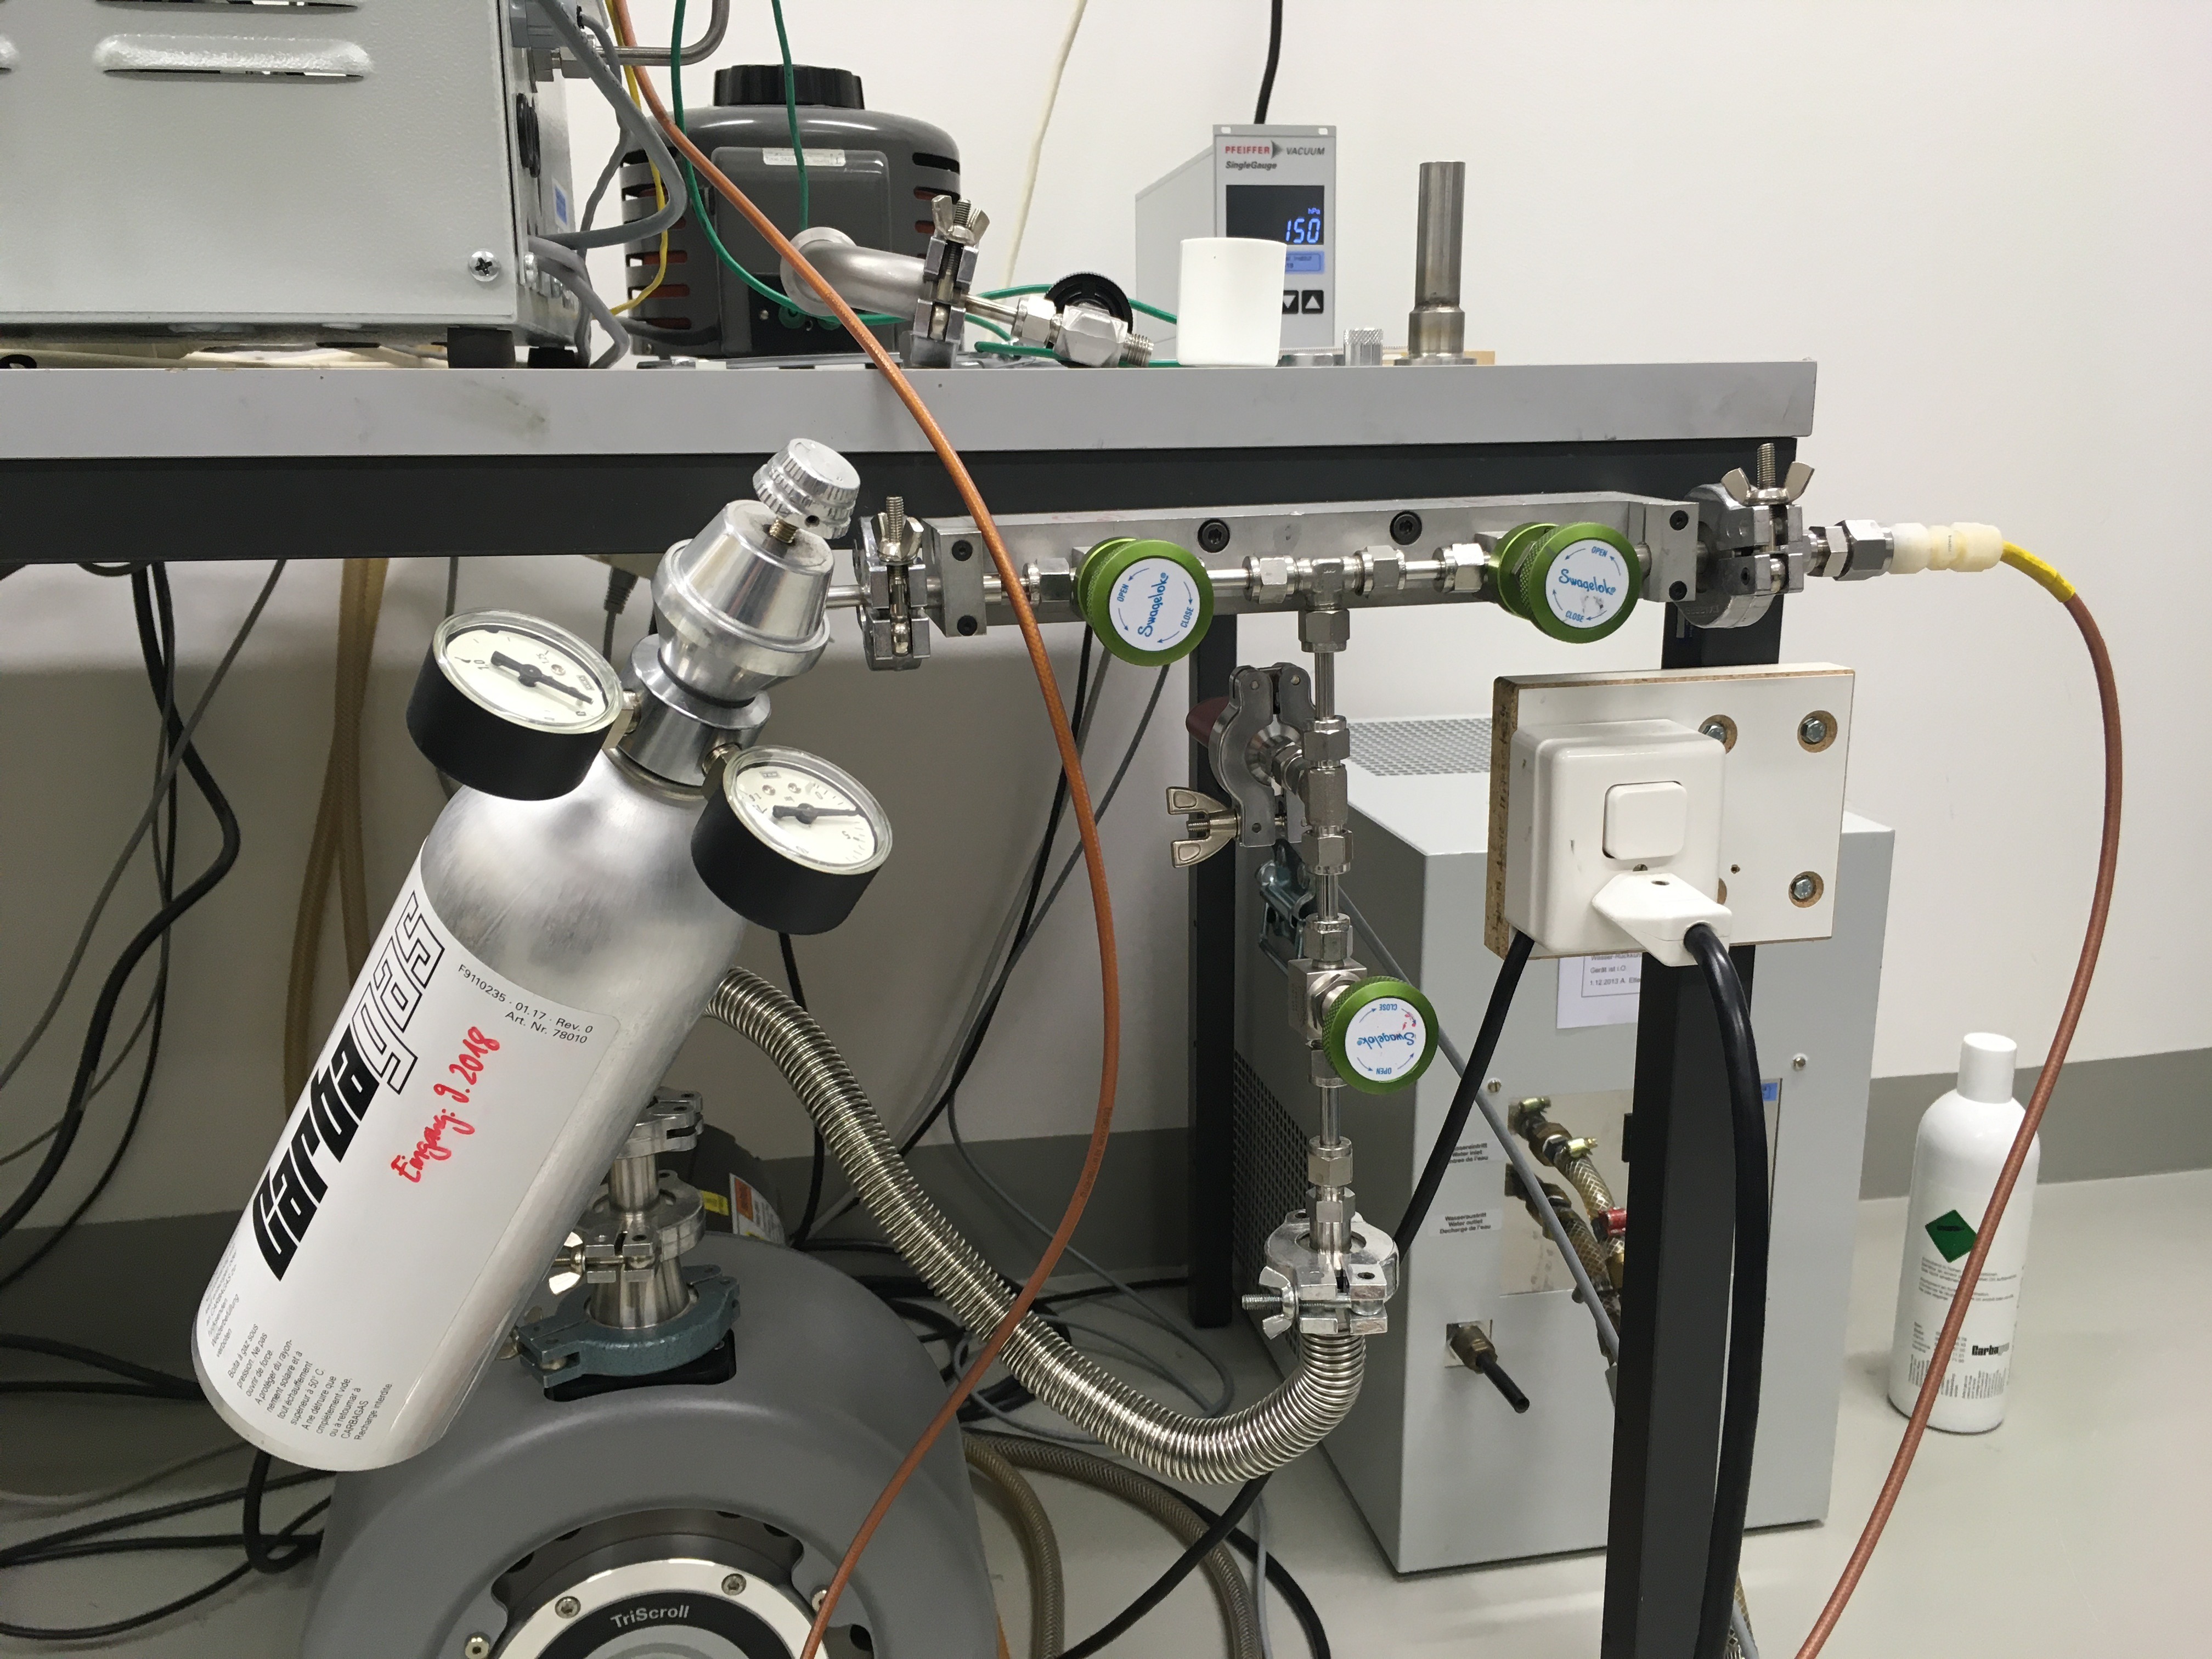
\includegraphics[width=0.5\textwidth]{Report/pictures/cartridge.JPG}
    \caption{The setup with an attached noble gas cartridge.}
    \label{fig:noblegas}
    \end{figure}
    
    \newpage
    \subsection{Inhaled Air}
    To compare the amount of carbon-dioxide and oxygen in exhaled air, one of us exhaled air into a balloon, attached it to the system and performed a measurement. Afterwards, one of us inhaled the air again and exhaled it again into the balloon. We repeated this procedure 5 times. The system was flushed with normal air in between each measurement. The peaks of carbon dioxide and oxygen were fitted using a {\scshape Gaussian} as described in section \ref{sec:fit}. The integrated data is normalised over the total data-set and is shown with uncertainties in figure \ref{fig:air}. 
    \begin{figure}[h!]
        \centering
        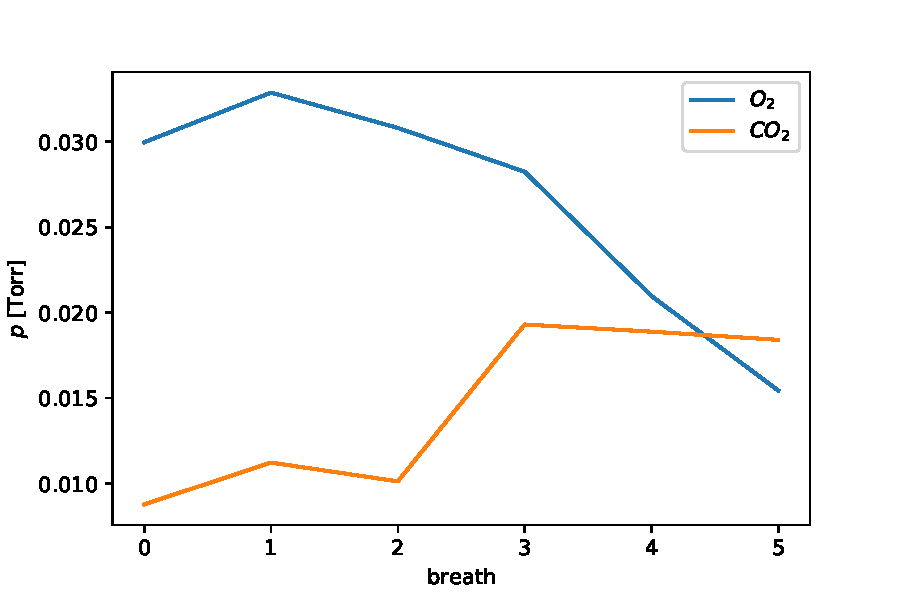
\includegraphics[width=0.6\textwidth]{Report/DataResultsPlots/air.pdf}
        \caption{CO$_2$ and O$_2$ amount in Inhaled air.}
        \label{fig:air}
    \end{figure}
    To get an estimation of how much oxygen is actually converted into carbon dioxide we fit \eqref{eq:breath} to the oxygen set and \eqref{eq:breath2} to the carbon dioxide set.
    \begin{align}
        f_{\text{O}_2}(n) &= n_{\text{O}_2} \cdot p_{\text{O}_2}^n \label{eq:breath}\\
        f_{\text{CO}_2}(n) &= n_{\text{CO}_2} - n_{\text{CO}_2} \cdot p_{\text{CO}_2}^n \label{eq:breath2}
    \end{align}
    We thus received the initial value of oxygen:
    $$ n_{\text{O}_2} = (1.58 \pm 0.16) \%$$
    And the stationary value of carbon dioxide:
    $$ n_{\text{CO}_2} = (0.69 \pm 0.21) \%$$
    Theoretically the factors $p_{\text{O}_2}$ and $p_{\text{CO}_2}$ should be identical because the conversion ratio is 1:1. However, because our mass-spectrometer cannot relatively measure the amount correctly because not all elements are equally well ionized. The factors $p_i$ we received from the fit are:
    $$p_{\text{O}_2} = (81.91 \pm 2.47) \;\text{per breath}$$
    $$p_{\text{CO}_2} = (53.29 \pm 23.24) \;\text{per breath}$$
    This would suggest that between 19 and 50 \% of the inhaled oxygen would be converted to carbon-dioxide during one breath.
    In reality, the oxygen amount decreases by about 4 to 5 \% per breath \cite{breath}.\\
    In figure \ref{fig:air} we also notice that the error-bars on the oxygen measurements are significantly larger than the ones for the carbon-dioxide measurements. This is another indication that the system has not the same sensitivity for both elements.
    
    
    \subsection{Measurement of Ethanol}
    
    
    A mass-spectrometer is only able to measure gaseous probes. Since Ethanol is liquid at room temperature, we had to attach a bent tube that is closed on the bottom after filling it with Ethanol. After attaching it, we heated it with our hands to increase the amount of gaseous Ethanol entering the system. The setup is shown in figure \ref{fig:ethanol}.
    \begin{figure}[h!]
    \centering
    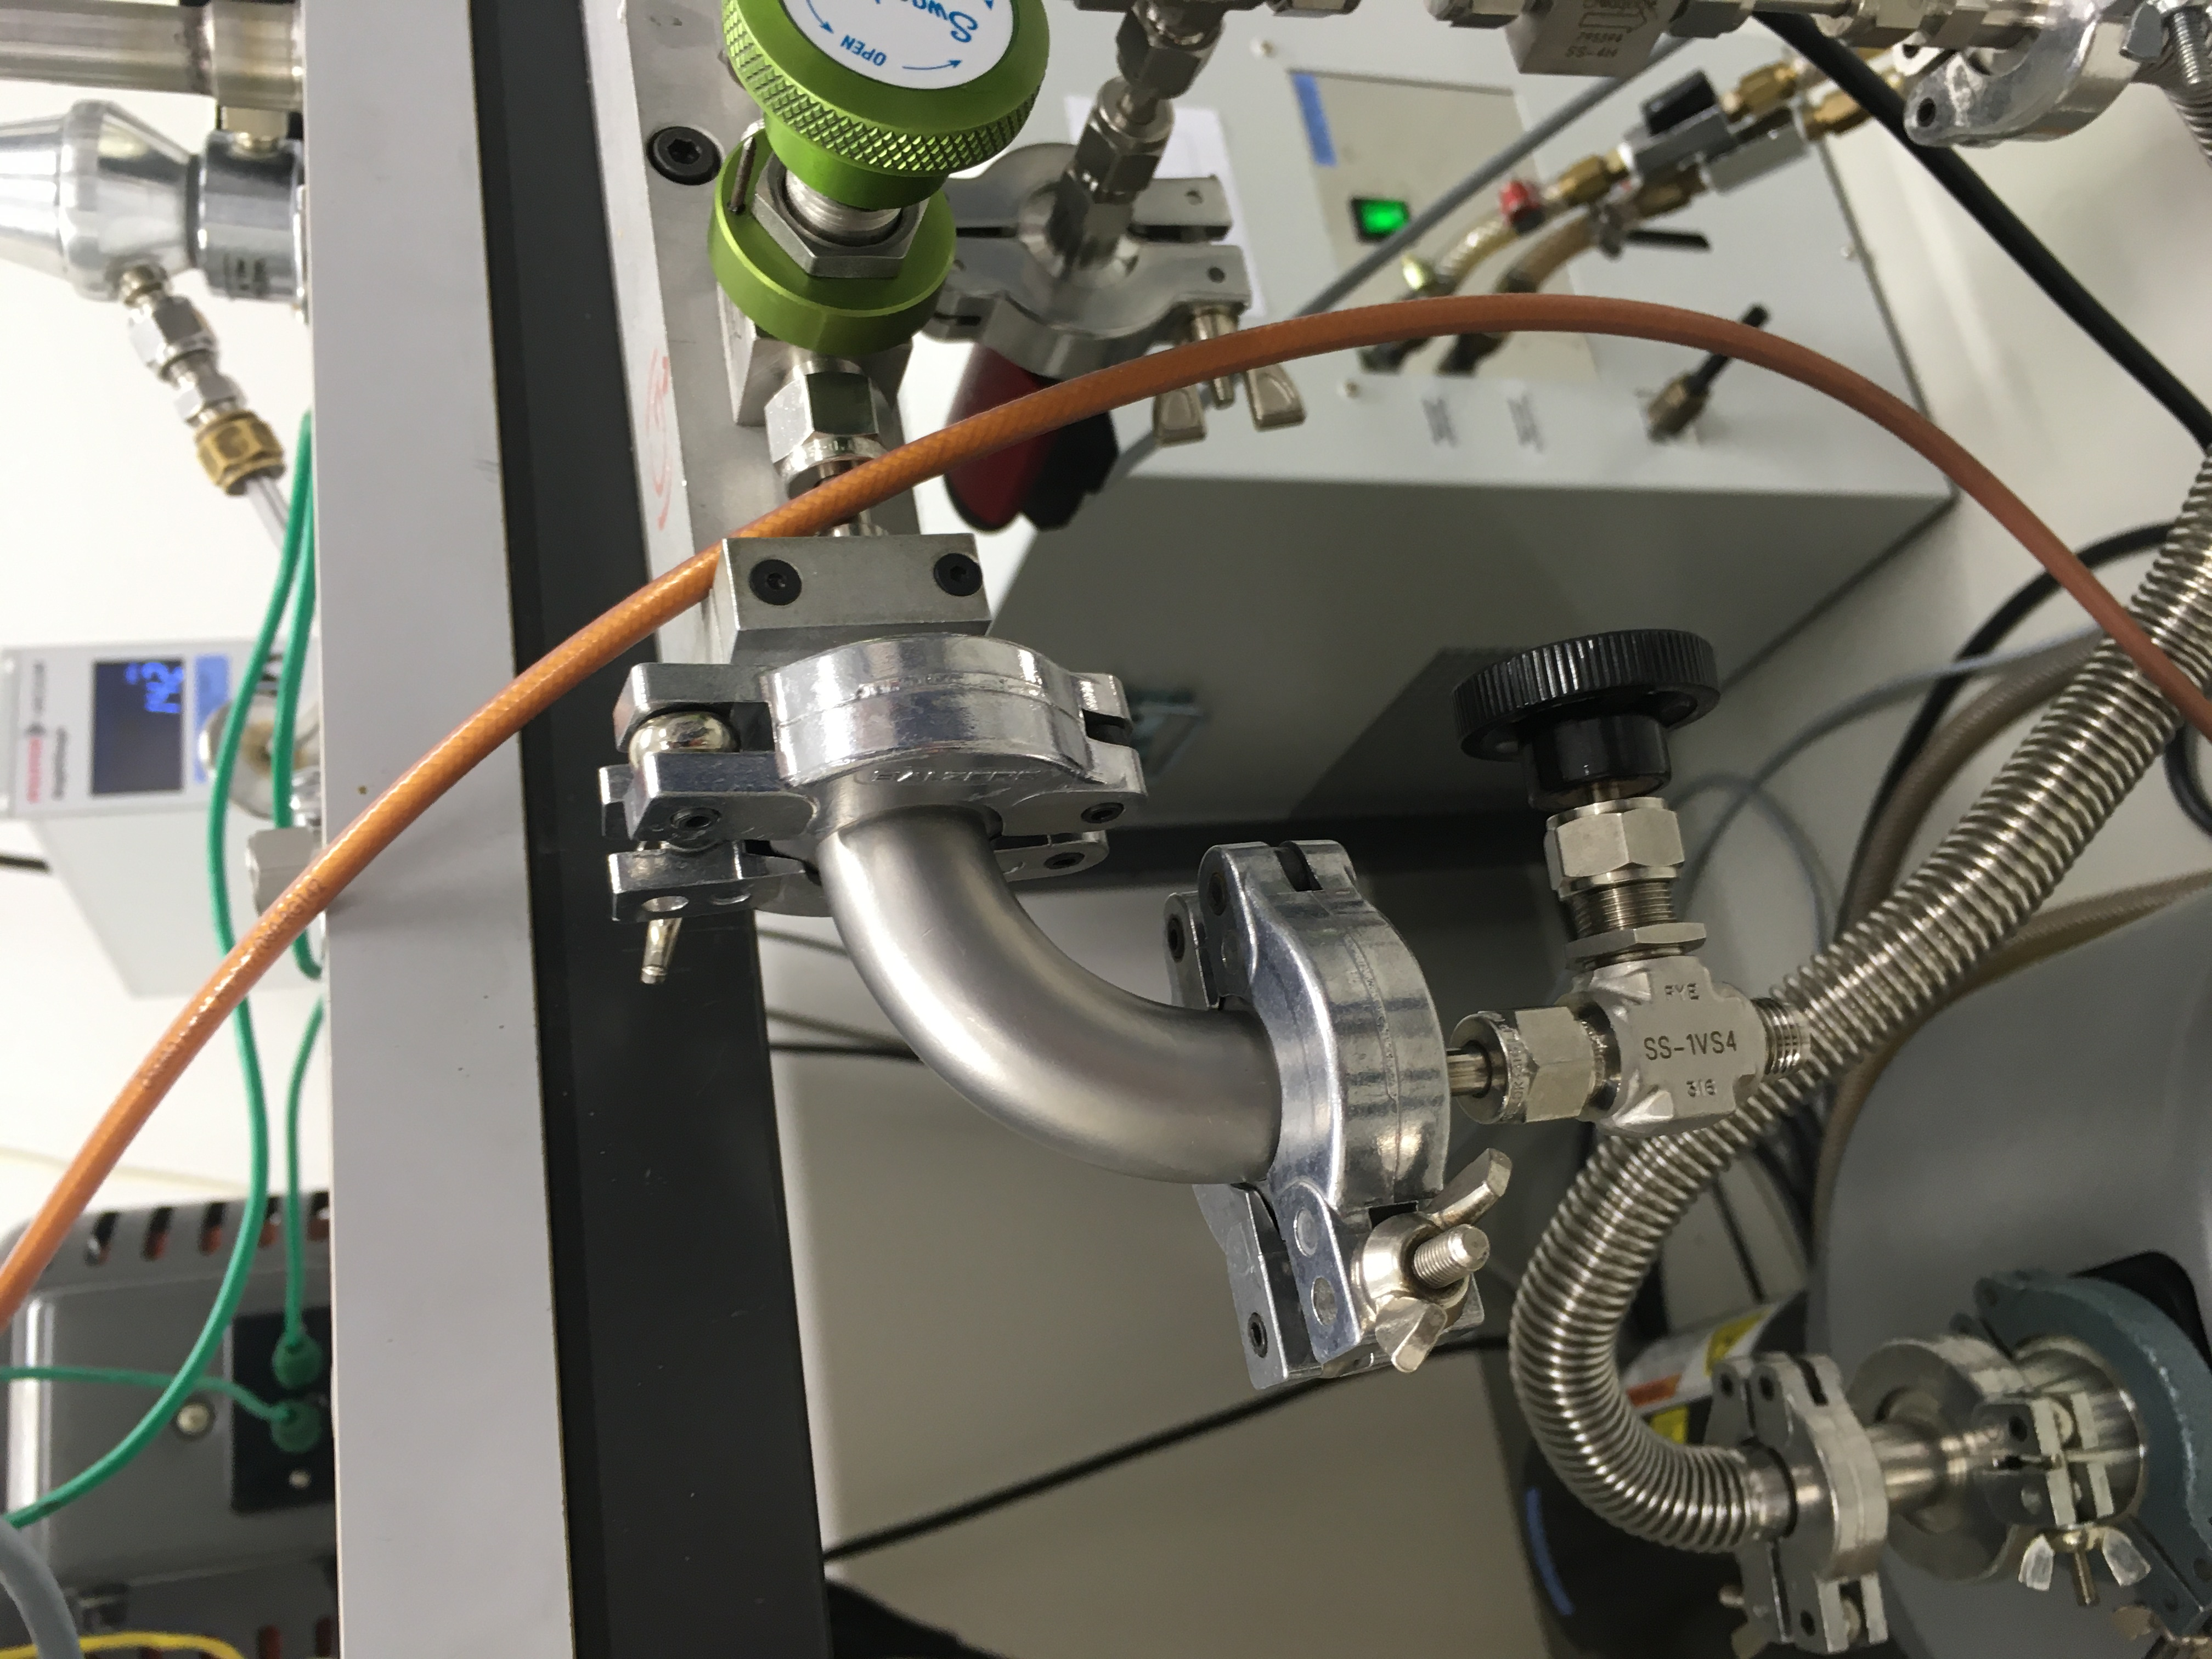
\includegraphics[angle=-90, origin=c, width=0.4\textwidth]{Report/pictures/liquids.JPG}
    \caption{The setup to attach a liquid sample to the system. The gaseous phase will be pumped to the mass spectrometer while the liquid phase will stay inside the container.}
    \label{fig:ethanol}
    \end{figure}
    The output of our measurements were compared to the literature value of NIST \cite{NIST} and are shown together in figure \ref{fig:ethanol2}.
    \begin{figure}[h!]
    \centering
    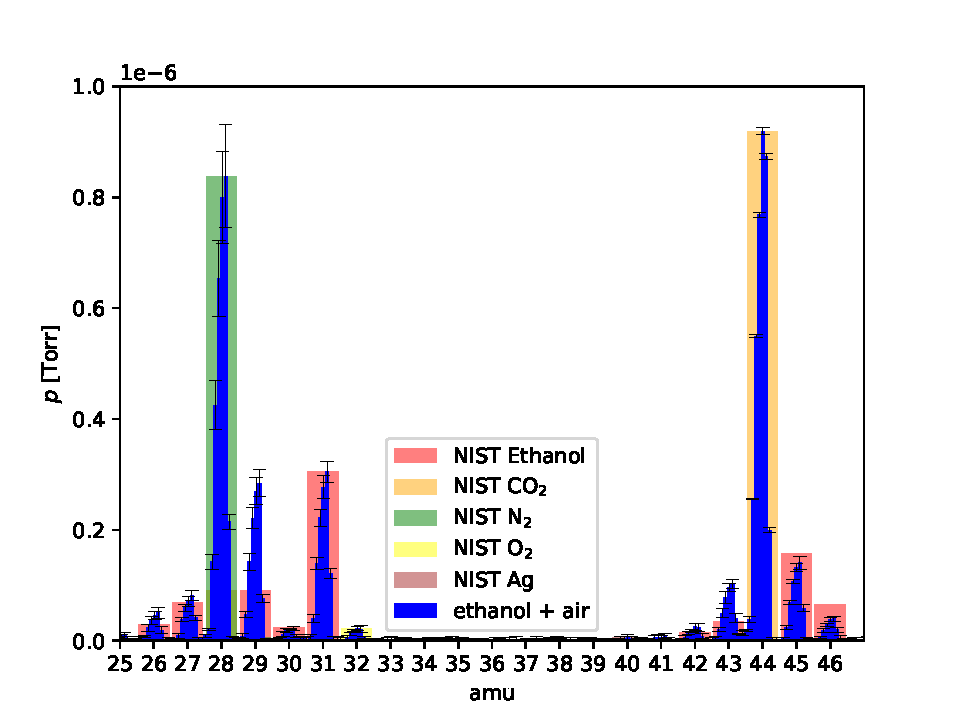
\includegraphics[angle=-90, origin=c, width=0.4\textwidth]{Report/DataResultsPlots/ethanol2.pdf}
    \caption{The measurements of our ethanol and air sample compared to NIST.}
    \label{fig:ethanol2}
    \end{figure}
    
    
    In addition to measuring ethanol and normal exhaled air, we exhaled air into a balloon just after having consumed some Vodka. The goal would have been to recognize the ethanol in the measurement. Sadly, the system is not sensitive enough to detect this small amounts.
    
    
    \newpage
    \subsection{Deo and Sparkling Water Analysis}
    
    \begin{figure}[h]
            \centering
            \subfloat[balloon with CO2 from sparkling water]{\label{figure:sparkling}
                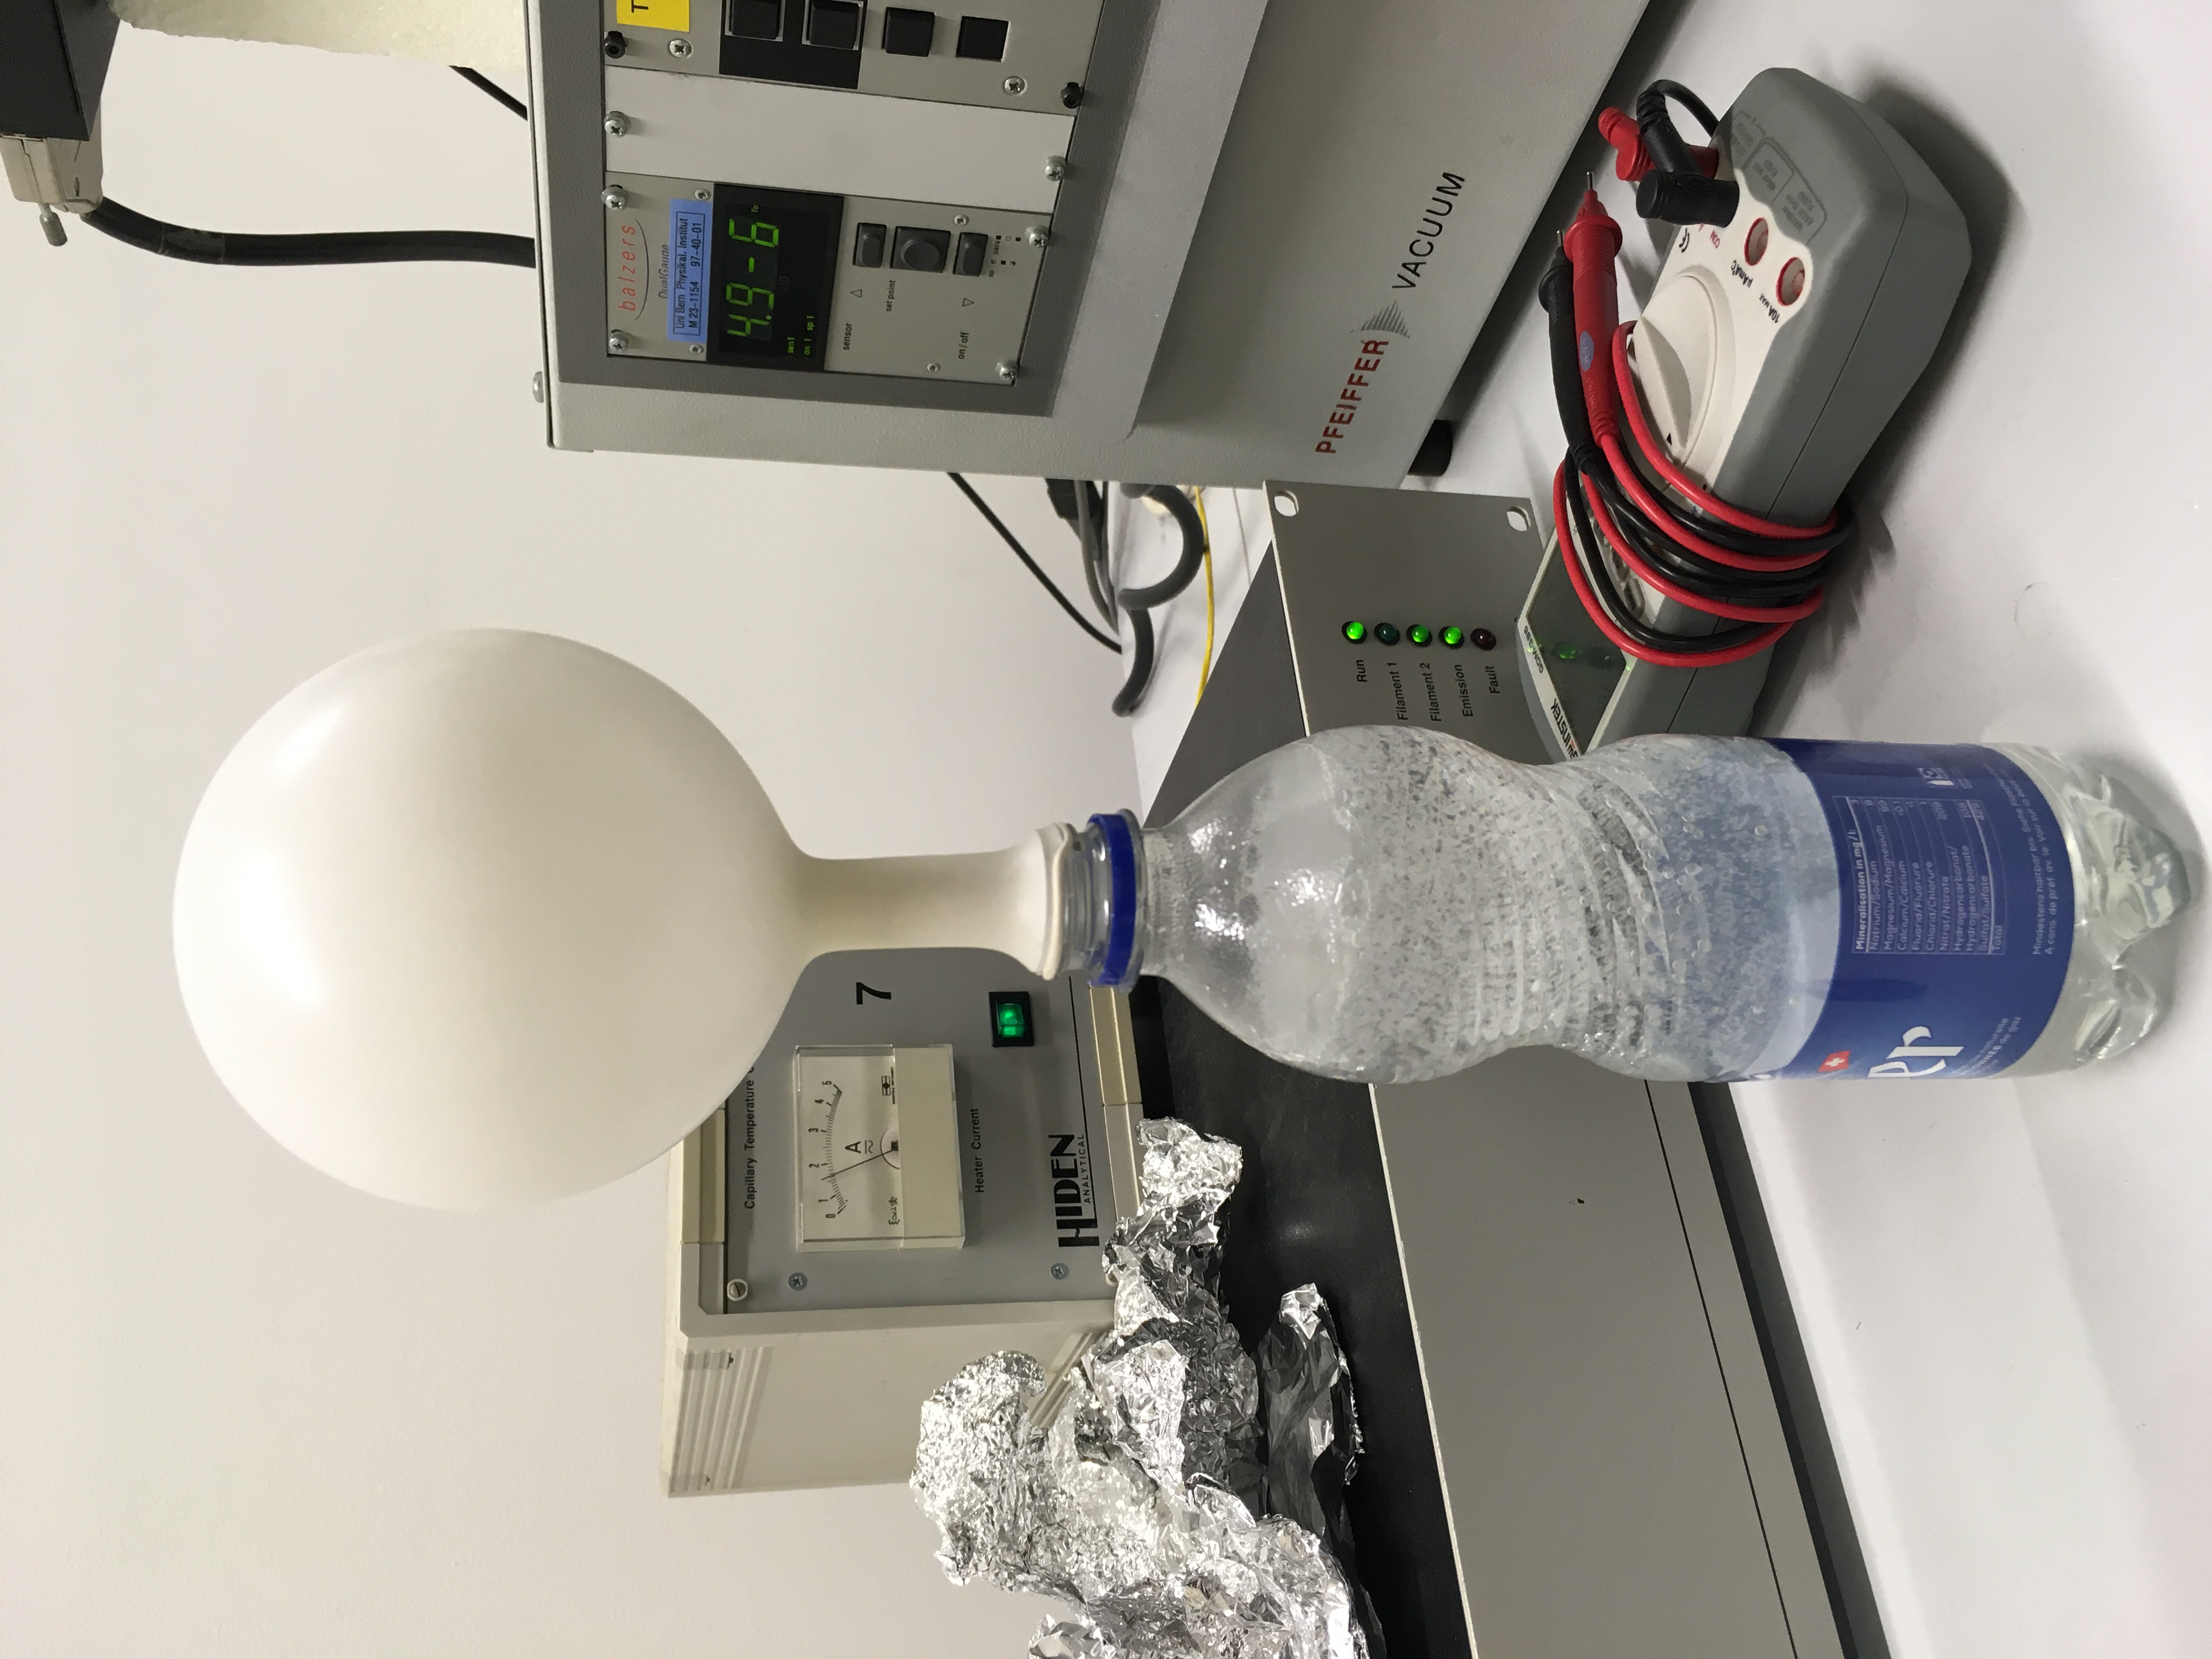
\includegraphics[width=0.47\textwidth, angle=270, origin=c]{Report/pictures/ballon_bottle2.JPG}}\quad
            \subfloat[balloon attached to the system]{\label{figuer:sparkling2}
                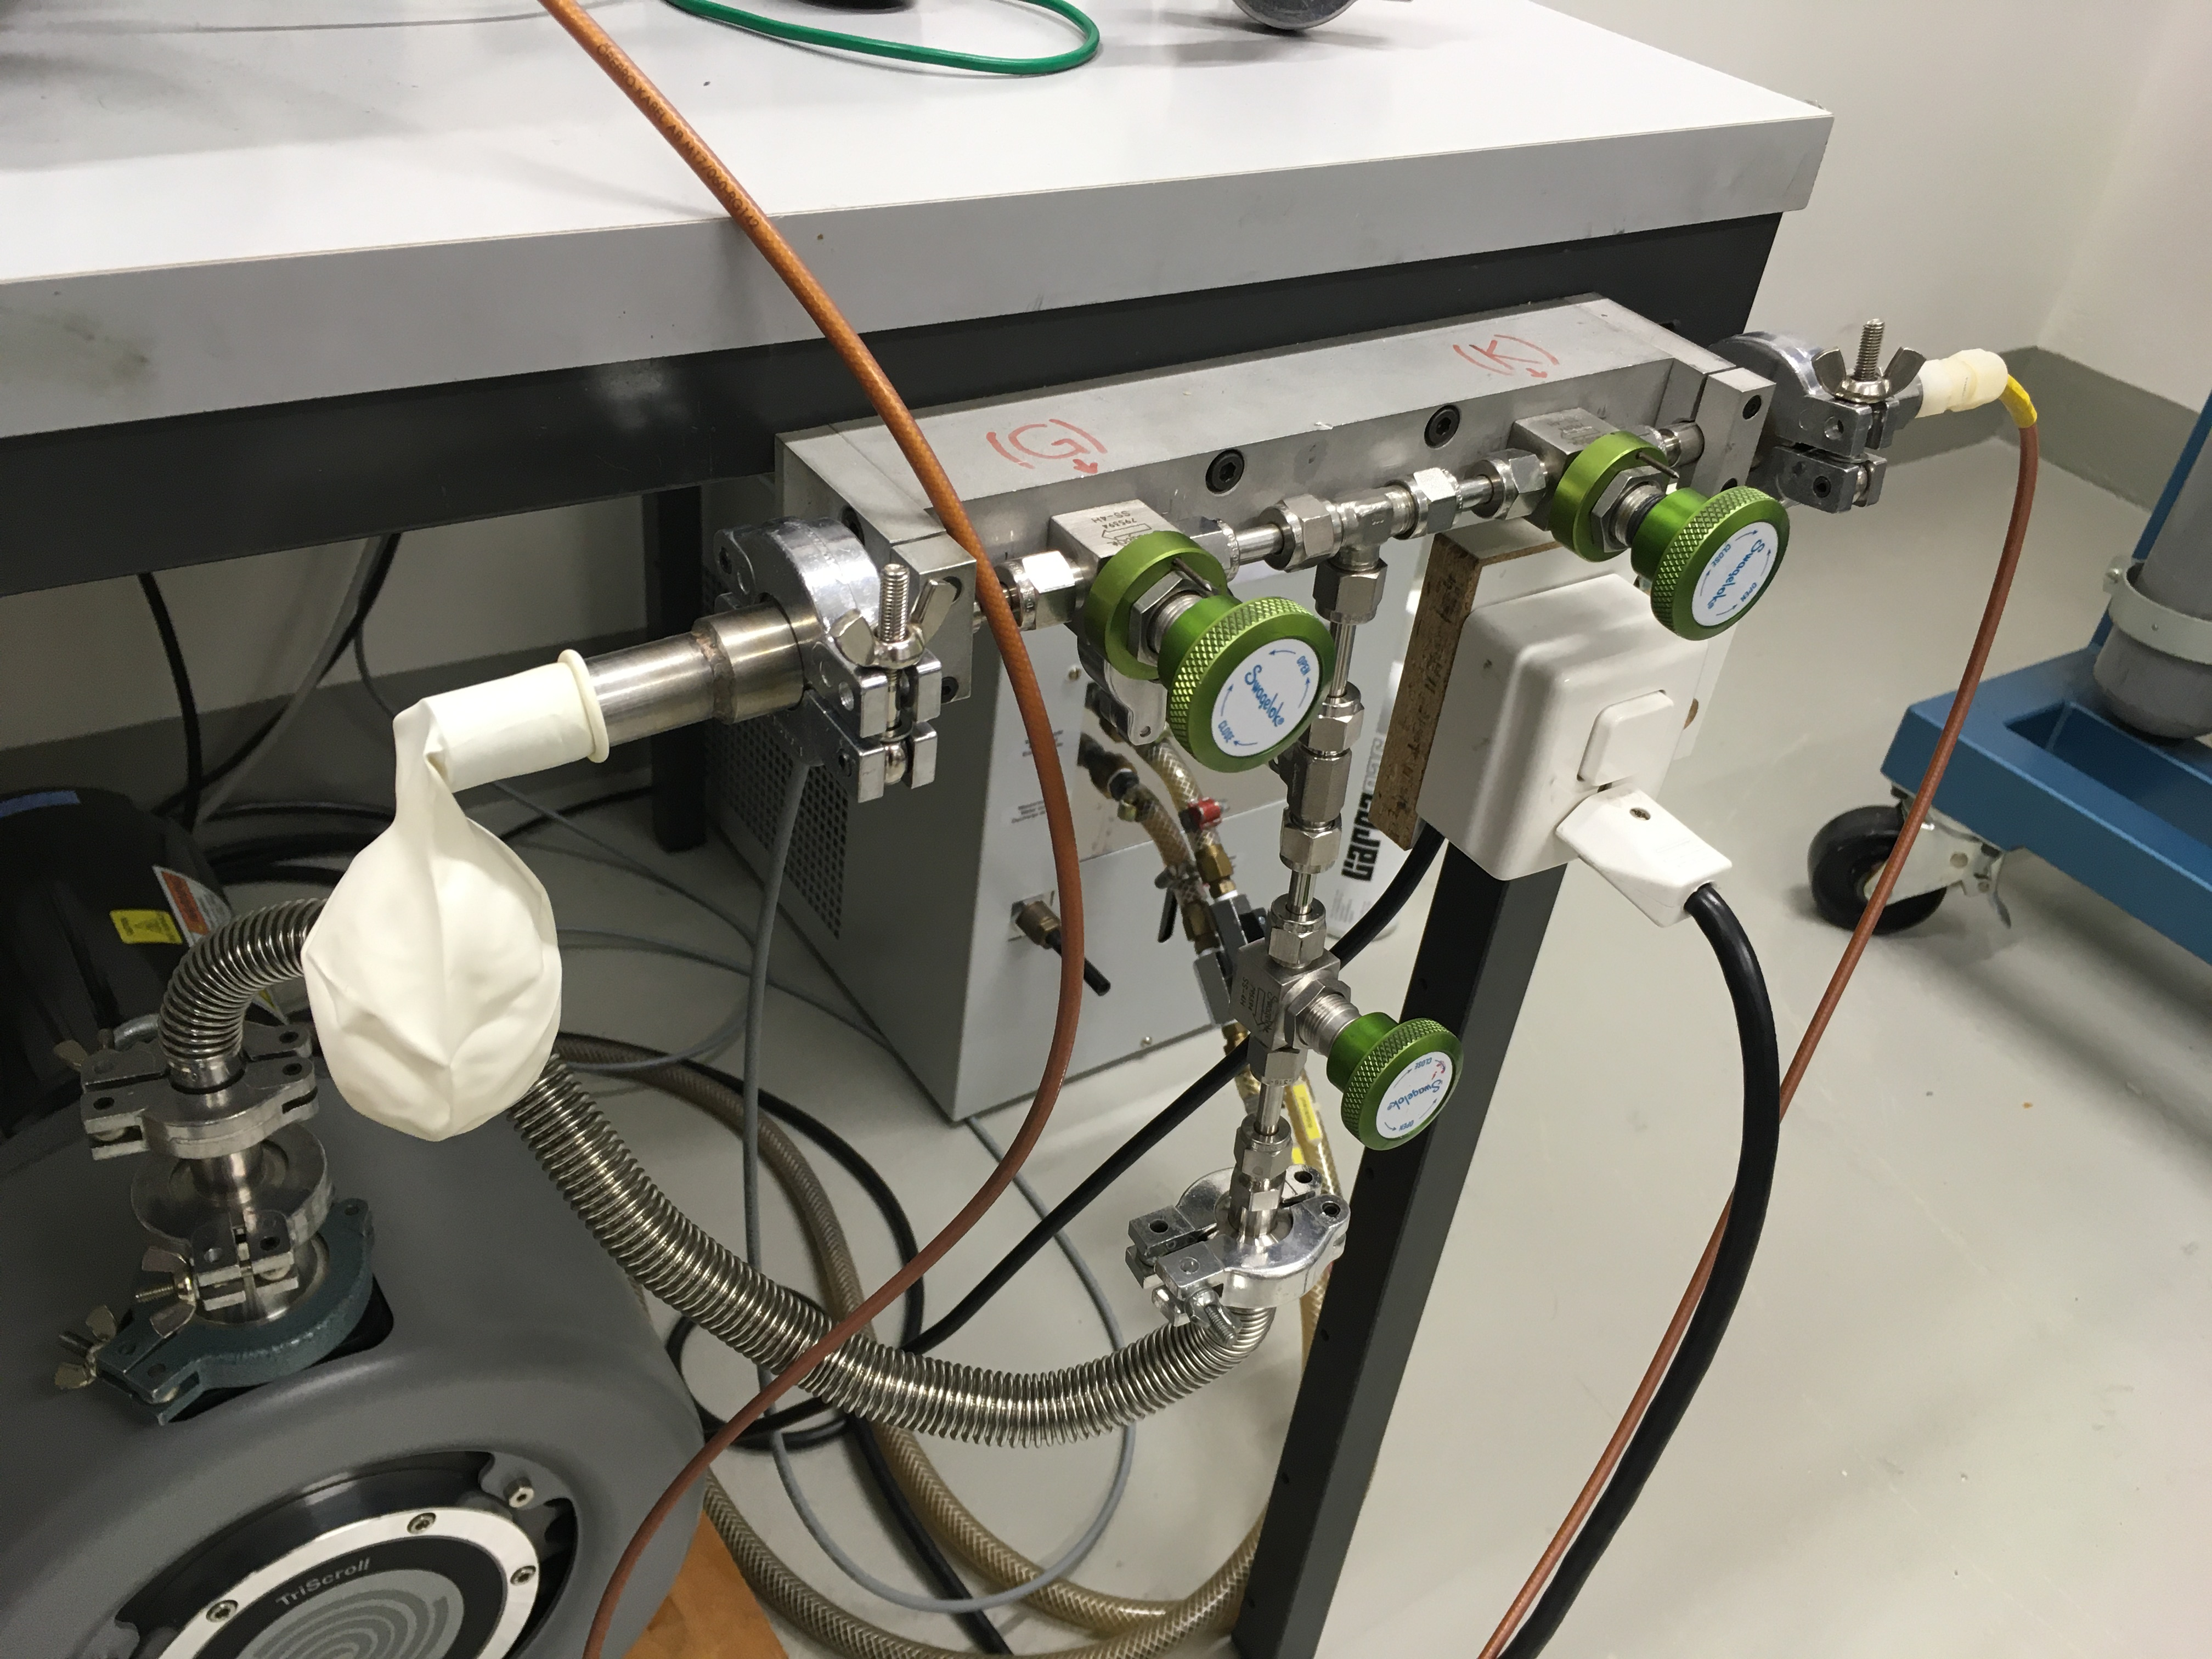
\includegraphics[width=0.47\textwidth]{Report/pictures/ballon_setup.JPG}}\quad
            \caption{The setup of the experiment with samples filled into a balloon.}
            \label{fig:setup2}
    \end{figure}